\chapter{Analiză și fundamentare teoretică}
\label{ch:analysis}
\pagestyle{fancy}

\section{Modelul conceptual al soluției}
\label{sec:model-conceptual-solutie}

Sistemul propus este un instrument de adnotare asistată, în care utilizatorul controlează rezultatul final, iar componentele automate produc propuneri inițiale.
O imagine de intrare $I$ este transformată într-o mulțime de adnotări:
\[
    A = \{a_1, a_2, \ldots, a_n\}.
\]
Fiecare adnotare conține un tip geometric, o etichetă semantică, o culoare de afișare și coordonate exprimate în sistemul imaginii originale.
Tipurile geometrice folosite sunt: dreptunghi de încadrare, poligon și mască.

Fluxul este de tip \textit{human-in-the-loop}: modelul propune, utilizatorul verifică și corectează.
Această alegere este importantă deoarece segmentarea automată poate produce contururi incomplete, etichete greșite sau obiecte false pozitive.
În loc să trateze predicția ca rezultat definitiv, aplicația o transformă într-o adnotare editabilă.
Astfel, viteza modelelor de inteligență artificială este combinată cu judecata adnotatorului.

\section{Algoritmi utilizați}
\label{sec:algoritmi-utilizati}

La nivel funcțional, aplicația folosește trei categorii de algoritmi: algoritmi de generare a adnotărilor vizuale, algoritmi de asistență conversațională și algoritmi de sincronizare colaborativă.
Această secțiune descrie rolul lor la nivel înalt, fără a intra în detalii de implementare.

\subsection{Algoritmul AutoSeg}
\label{subsec:algoritm-autoseg}

AutoSeg este algoritmul folosit pentru detecție și segmentare automată la nivelul întregii imagini.
Intrările sale sunt imaginea curentă, lista de clase urmărite și un prag minim de încredere.
Ieșirea este o listă de obiecte candidate, fiecare obiect putând conține o etichetă, un scor, o cutie de încadrare și un contur de segmentare.

Pașii logici ai algoritmului sunt:
\begin{enumerate}
    \item utilizatorul alege clasele sau etichetele de interes;
    \item imaginea este analizată de modelul extern;
    \item predicțiile cu scor sub pragul ales sunt eliminate;
    \item pentru fiecare predicție validă se extrage dreptunghiul de încadrare și, dacă există, masca obiectului;
    \item rezultatul este convertit într-o adnotare editabilă.
\end{enumerate}

O predicție AutoSeg poate fi reprezentată abstract prin:
\[
    d_i = (label_i, score_i, bbox_i, mask_i).
\]
Componenta $bbox_i$ localizează rapid obiectul, iar $mask_i$ descrie conturul său.
Dacă masca nu este disponibilă, dreptunghiul de încadrare rămâne o reprezentare minimă utilă.
Avantajul algoritmului este că poate genera mai multe adnotări într-o singură rulare.
Limitarea sa este dependența de modelul vizual și de compatibilitatea dintre etichetele cerute și obiectele pe care modelul le poate recunoaște.

\subsection{Algoritmul AutoMask}
\label{subsec:algoritm-automask}

AutoMask este algoritmul folosit pentru segmentare interactivă.
Spre deosebire de AutoSeg, care caută obiecte în întreaga imagine, AutoMask pornește de la un indiciu spațial oferit de utilizator.
Cel mai simplu indiciu este un punct $p=(x,y)$ ales în interiorul regiunii de interes.
Modelul returnează o mască $M$ asociată acelei regiuni:
\[
    f(I, p) \rightarrow M.
\]

În modul de segmentare completă, algoritmul poate produce mai multe măști candidate:
\[
    f(I) \rightarrow \{M_1, M_2, \ldots, M_m\}.
\]
Acest mod este util când imaginea conține mai multe obiecte sau regiuni care pot fi pre-adnotate în bloc.

După generarea măștii, aplicația normalizează rezultatul pentru afișare și editare.
Normalizarea urmărește două obiective: păstrarea formei relevante a obiectului și reducerea costului de randare.
Această etapă este necesară deoarece o mască brută poate conține un număr foarte mare de puncte, iar manipularea ei directă poate încetini interfața.

\subsection{Algoritmul de asistență LLM}
\label{subsec:algoritm-llm}

Asistentul local folosește modele lingvistice mari pentru dialog cu utilizatorul.
Rolul său nu este să modifice automat adnotările, ci să explice pași, să ajute la depanare și să ofere recomandări în fluxul de lucru.
Conversația este reprezentată ca o listă de mesaje cu roluri: sistem, utilizator și asistent.

Un model lingvistic autoregresiv estimează următorul token pe baza contextului deja generat:
\[
    P(t_n \mid t_1, t_2, \ldots, t_{n-1}).
\]
Răspunsul este produs iterativ, token cu token.
Parametrii precum dimensiunea contextului, temperatura, \textit{top-p} și numărul maxim de tokeni controlează lungimea, variația și predictibilitatea răspunsului.
În aplicație sunt folosite două moduri locale de rulare: \texttt{llama.cpp}, prin \texttt{llama-cpp-python}, și Ollama, prin client local.

\subsection{Algoritmul de sincronizare colaborativă}
\label{subsec:algoritm-colaborativ}

Pentru colaborare, aplicația tratează modificările ca evenimente.
Crearea, actualizarea și ștergerea unei adnotări sunt reprezentate prin mesaje care modifică starea sesiunii.
Această stare poate fi descrisă prin relația:
\[
    S_{v+1} = apply(S_v, e),
\]
unde $S_v$ este starea sesiunii la versiunea $v$, iar $e$ este evenimentul primit.
Versiunea incrementală ajută la ignorarea evenimentelor vechi, iar identificatorul unic al evenimentului ajută la eliminarea duplicatelor.

Protocolul STOMP peste WebSocket este potrivit pentru acest flux deoarece permite modelul publicare/abonare: un client trimite un eveniment, iar ceilalți clienți abonați la aceeași sesiune îl primesc aproape în timp real.
Prin această abordare, adnotările manuale și cele generate de AutoSeg sau AutoMask sunt sincronizate uniform.

\section{Modele de inteligență artificială folosite}
\label{sec:modele-ai-folosite}

Algoritmii descriși anterior sunt susținuți de trei familii de modele: YOLO pentru detecție și segmentare, Mask2Former pentru segmentare externă și modele lingvistice bazate pe Transformer pentru asistența locală.

\subsection{YOLO pentru AutoSeg}
\label{subsec:model-yolo-autoseg}

YOLO tratează detecția obiectelor ca o problemă de predicție directă.
În loc să genereze mai întâi regiuni candidate și apoi să le clasifice separat, modelul procesează imaginea într-o singură trecere și prezice simultan poziția obiectelor, clasa lor și scorul de încredere.
Imaginea este transformată într-o hartă de caracteristici, iar pe baza acesteia modelul estimează pentru fiecare obiect coordonatele cutiei de încadrare și probabilitatea apartenenței la o clasă.
În variantele cu segmentare, aceeași predicție este completată cu informații despre masca obiectului.
Pentru o aplicație de adnotare, această abordare este utilă deoarece reduce timpul dintre acțiunea utilizatorului și apariția propunerilor pe canvas.

În AutoSeg, modelul YOLO este folosit ca mecanism de pre-adnotare.
Utilizatorul indică etichetele urmărite, iar modelul analizează întreaga imagine și întoarce o listă de obiecte candidate.
Fiecare rezultat poate fi transformat fie într-un dreptunghi de încadrare, fie într-un poligon sau mască, în funcție de informațiile disponibile.
Astfel, modelul nu este tratat ca un modul care decide definitiv adnotarea, ci ca un generator de propuneri care accelerează munca utilizatorului.

YOLOE extinde principiul YOLO către detecție și segmentare \textit{open-vocabulary}, adică permite lucrul cu clase descrise prin prompturi textuale sau vizuale, nu doar cu o listă fixă de clase~\cite{wang2025yoloerealtimeseeing}.
Arhitectura sa combină un extractor de caracteristici, o structură de agregare multi-scală de tip PAN și capete de predicție pentru regresie, segmentare și embedding.
Prin alinierea dintre reprezentările vizuale și cele textuale, modelul poate răspunde la cereri mai flexibile decât un detector antrenat strict pe un set închis de categorii.

\begin{figure}[ht]
    \centering
    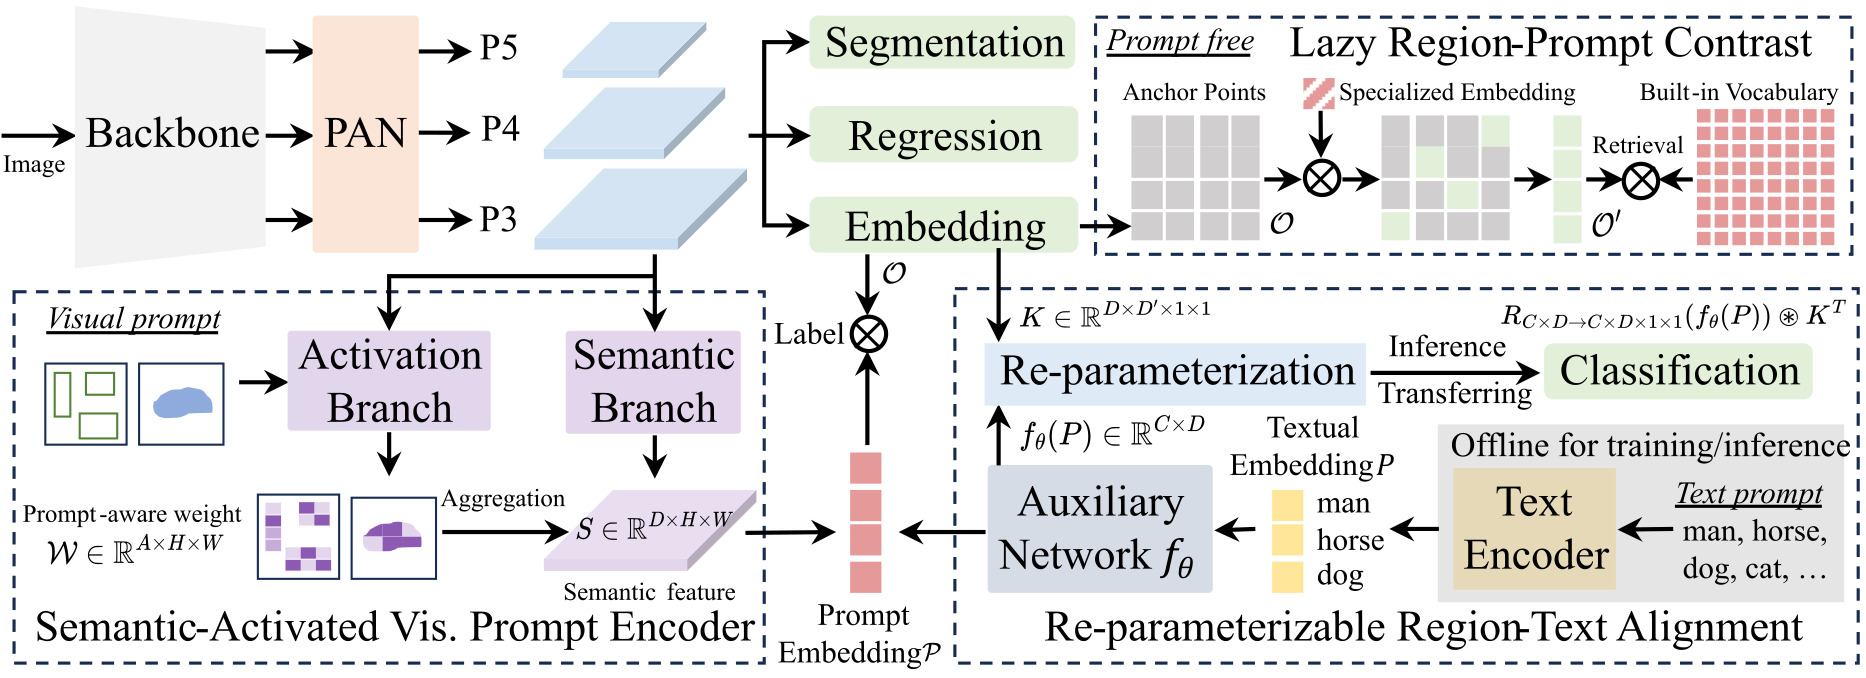
\includegraphics[width=\textwidth]{figs/yoloe.jpg}
    \caption{Arhitectura YOLOE folosită ca reper pentru AutoSeg}
    \label{fig:yoloe-architecture}
\end{figure}

În figura~\ref{fig:yoloe-architecture} se observă separarea dintre extragerea de caracteristici, agregarea multi-scală și capetele de predicție.
Pentru aplicația de adnotare, elementul relevant nu este antrenarea modelului, ci forma rezultatului: o listă de obiecte candidate care pot deveni adnotări editabile.
YOLOE ajută proiectul prin caracterul său generalist: același tip de model poate fi folosit pentru mai multe clase și contexte vizuale, fără ca interfața de adnotare să fie proiectată pentru un singur domeniu.
Această flexibilitate susține scopul aplicației, deoarece utilizatorul poate lucra cu imagini variate și poate folosi AutoSeg ca punct de pornire rapid, urmat de corecție manuală.

\subsection{Mask2Former pentru AutoMask}
\label{subsec:model-mask2former-automask}

Mask2Former este folosit ca fundament pentru AutoMask deoarece problema principală aici nu este doar localizarea obiectului, ci obținerea unei regiuni precise.
Modelul formulează segmentarea ca predicție de măști și poate aborda segmentarea semantică, segmentarea de instanțe și segmentarea panoptică folosind aceeași arhitectură generală~\cite{cheng2022maskedattentionmasktransformeruniversal}.
Această proprietate este importantă pentru aplicație: indiferent dacă utilizatorul urmărește o regiune semantică sau un obiect individual, rezultatul util este tot o mască editabilă.

Arhitectura poate fi înțeleasă în trei etape.
Prima etapă este extragerea caracteristicilor vizuale printr-un \textit{backbone}.
Acesta transformă imaginea într-o reprezentare internă care conține informații despre texturi, muchii, forme și obiecte.
A doua etapă este \textit{pixel decoder}-ul, care reconstruiește informația spațială necesară pentru segmentare la rezoluții utile.
A treia etapă este decodorul Transformer, care lucrează cu interogări de obiect și produce predicții de clasă și măști.

Elementul central al Mask2Former este mecanismul de \textit{masked attention}.
În loc ca fiecare interogare să acorde atenție întregii imagini, atenția este restrânsă la regiuni candidate.
Această restrângere reduce influența fundalului și permite rafinarea progresivă a conturului.
Pentru AutoMask, acest lucru este util deoarece un punct selectat de utilizator poate fi transformat într-o regiune coerentă, iar regiunea rezultată poate fi corectată ulterior prin instrumentele de editare.

\begin{figure}[ht]
    \centering
    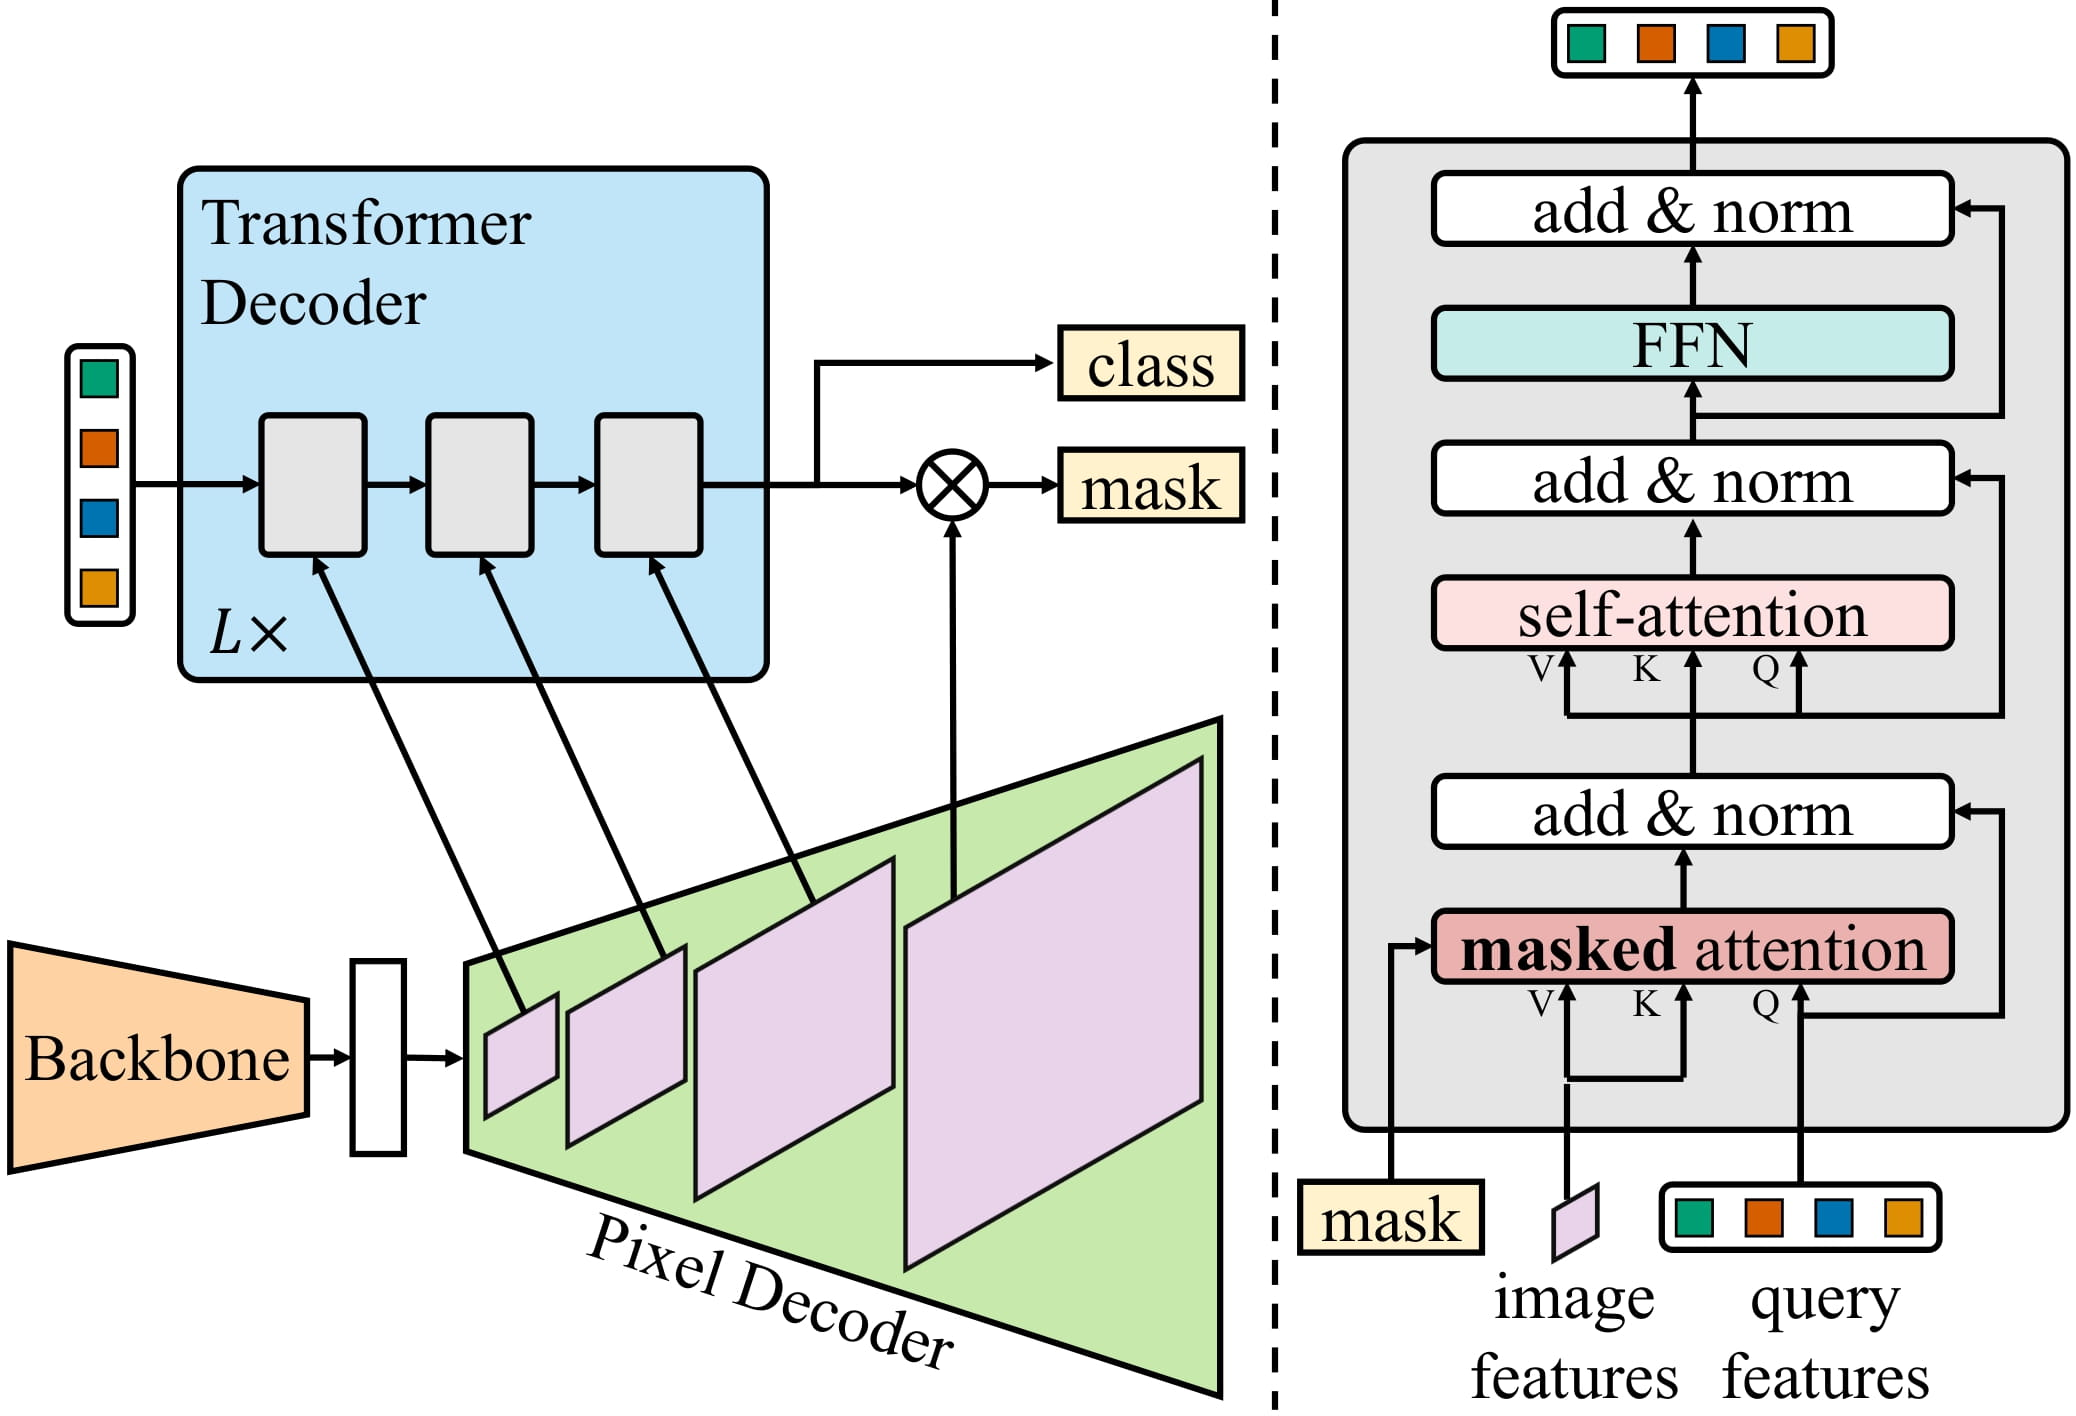
\includegraphics[width=0.92\textwidth]{figs/mask2former_architecture.jpg}
    \caption{Arhitectura Mask2Former pentru predicția măștilor}
    \label{fig:mask2former-architecture}
\end{figure}

În figura~\ref{fig:mask2former-architecture}, masca nu este doar un rezultat final, ci și un element folosit în atenția modelului.
Această proprietate explică de ce Mask2Former este potrivit pentru generarea unor contururi inițiale care pot fi apoi corectate de utilizator.
În proiect, AutoMask valorifică exact acest comportament: modelul extern produce o mască, iar aplicația o transformă într-o adnotare manipulabilă în canvas.

\subsection{Modele lingvistice bazate pe Transformer}
\label{subsec:model-transformer-llm}

Modelele LLM folosite de aplicație sunt bazate pe arhitectura Transformer, introdusă ca mecanism de procesare secvențială prin atenție~\cite{vaswani2017attentionneed}.
În modelele conversaționale moderne, varianta de tip \textit{decoder-only} este folosită frecvent pentru generare autoregresivă.
Modelul primește istoricul conversației, calculează relații de atenție între tokeni și produce următorul token.

\begin{figure}[ht]
    \centering
    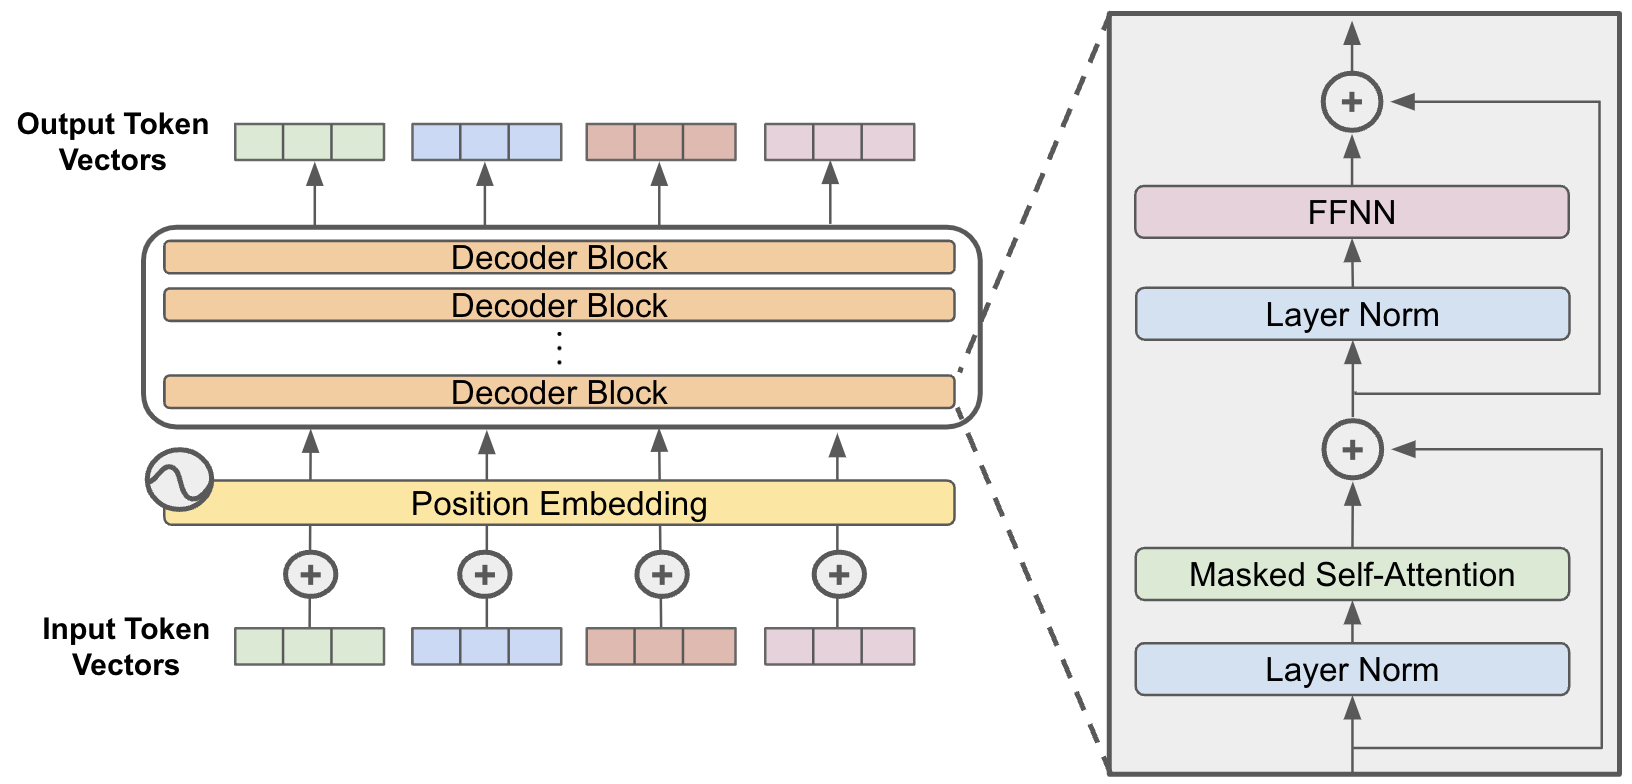
\includegraphics[width=0.92\textwidth]{figs/transformer_decoder_only.png}
    \caption{Structură generală de model Transformer de tip decoder-only}
    \label{fig:transformer-decoder-only}
\end{figure}

În figura~\ref{fig:transformer-decoder-only}, blocurile principale sunt embedding-ul pozițional, atenția mascată, normalizarea și rețeaua feed-forward.
Atenția mascată împiedică modelul să folosească tokeni viitori în timpul generării, menținând caracterul autoregresiv.

În proiect există două variante de rulare locală.
\texttt{llama.cpp} permite încărcarea directă a unui model local și controlul parametrilor de inferență~\cite{llamacpp2026}.
Ollama oferă un serviciu local care gestionează modelele disponibile și expune o interfață simplă pentru conversație~\cite{ollama2026}.
Ambele variante susțin aceeași decizie arhitecturală: asistența conversațională rulează local, fără a trimite datele aplicației către un serviciu cloud.

\section{Protocoale utilizate}
\label{sec:protocoale-utilizate}

Aplicația folosește protocoale diferite pentru tipuri diferite de comunicare.
Operațiile punctuale, precum autentificarea sau obținerea stării unei sesiuni, sunt tratate prin HTTP (Hypertext Transfer Protocol)/REST.
Comunicarea continuă, precum chatul și sincronizarea adnotărilor, folosește WebSocket peste care este aplicat STOMP.
Evenimentele interne dintre servicii sunt transmise prin RabbitMQ, folosind AMQP (Advanced Message Queuing Protocol).
Astfel, fiecare protocol este folosit acolo unde se potrivește natural: cerere-răspuns, timp real sau mesagerie asincronă.

\subsection{HTTP/REST}
\label{subsec:http-rest}

HTTP/REST este folosit pentru acțiuni discrete, unde clientul trimite o cerere și primește un răspuns complet.
În proiect, acest protocol acoperă autentificarea, înregistrarea utilizatorilor, validarea tokenului JWT, listarea sesiunilor, crearea sesiunilor și obținerea snapshotului unei camere colaborative.
Este folosit și pentru transferul imaginilor temporare, deoarece fișierele imagine sunt mai potrivite pentru cereri HTTP decât pentru mesaje WebSocket.

JWT înseamnă \textit{JSON Web Token} și reprezintă un token semnat care transportă identitatea utilizatorului între client și server.
În proiect, el este emis după autentificare și este trimis ulterior la cererile protejate, astfel încât utilizatorul să nu retrimită parola la fiecare operație.
Structura sa este împărțită conceptual în trei părți: header, payload și semnătură.
Headerul descrie tipul tokenului și algoritmul folosit, payload-ul conține informațiile despre utilizator, iar semnătura permite verificarea integrității tokenului.
Această structură este ilustrată în figura~\ref{fig:jwt-structure}.

\begin{figure}[ht]
    \centering
    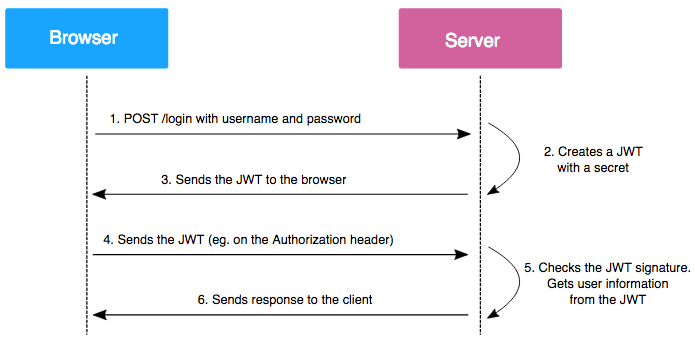
\includegraphics[width=0.82\textwidth]{figs/jwt-diagram.png}
    \caption{Structura generală a unui token JWT}
    \label{fig:jwt-structure}
\end{figure}

La nivel conceptual, REST reprezintă stratul de inițializare și recuperare.
El oferă clientului starea de pornire, iar după aceea sincronizarea continuă poate fi făcută prin canalul de timp real.
Această separare este importantă deoarece nu toate operațiile aplicației au nevoie de comunicare permanentă.
Autentificarea, încărcarea unei imagini sau cererea unui snapshot sunt operații finite, iar HTTP oferă un model clar pentru confirmarea succesului sau semnalarea erorilor.

În plus, REST creează un punct stabil de integrare între clientul desktop și serviciile backend.
Clientul nu trebuie să cunoască starea internă a serverului, ci doar resursele pe care le poate cere sau modifica.
Această abordare face ca pornirea unei sesiuni colaborative să fie predictibilă: mai întâi se obține starea inițială prin HTTP, apoi modificările live sunt primite prin WebSocket.

\subsection{WebSocket și STOMP}
\label{subsec:websocket-stomp}

WebSocket este folosit pentru comunicare persistentă între client și server.
Acest lucru este necesar pentru funcțiile care trebuie actualizate imediat: chat, prezență și sincronizarea adnotărilor.

STOMP înseamnă \textit{Simple Text Oriented Messaging Protocol} și definește un format simplu de mesaje trimise peste o conexiune, inclusiv operații de tip trimitere și abonare.
În proiect, este folosit peste WebSocket pentru a organiza mesajele pe destinații, astfel încât serverul să poată publica evenimente către topicuri sau cozi.
Specificația protocolului este disponibilă la \cite{stomp_spec_1_2}.

În aplicație, acest model permite separarea între mesaje globale și mesaje private.
Evenimentele de colaborare sunt trimise către camera de lucru, iar mesajele de chat sunt livrate utilizatorilor implicați în conversație.
Pentru adnotări mari, cum sunt măștile, sistemul poate fragmenta payload-ul și îl poate reasambla pe server, păstrând același model de eveniment.
Avantajul principal al WebSocket este latența redusă.
Într-o aplicație de adnotare colaborativă, un utilizator trebuie să vadă rapid modificările făcute de alt participant, altfel apar conflicte sau decizii luate pe o stare veche.
Canalul persistent permite transmiterea evenimentelor imediat ce apar, fără interogări repetate către server.

\subsection{SockJS ca fallback}
\label{subsec:sockjs}

SockJS este disponibil ca fallback pentru endpointurile WebSocket.
Rolul său este să permită conectarea și în medii unde WebSocket direct nu este disponibil sau este restricționat.
Pentru clientul desktop scenariul principal rămâne WebSocket nativ, dar suportul SockJS face backend-ul mai ușor de reutilizat de alte interfețe viitoare.
În proiect, SockJS este configurat în serviciile de chat și adnotare, la același endpoint WebSocket, ca alternativă de transport.
Fiind plasat la nivelul transportului, nu schimbă modelul de colaborare și nici formatul evenimentelor.
Această alegere este utilă deoarece serviciile backend nu rămân dependente de un singur tip de client.

\subsection{AMQP și RabbitMQ}
\label{subsec:amqp-rabbitmq}

AMQP, prin RabbitMQ, este folosit pentru evenimente asincrone între servicii.
În proiect, autentificarea poate publica evenimente interne, iar celelalte servicii le pot consuma fără apeluri directe între module.
Acest model reduce cuplarea dintre servicii: un serviciu anunță că s-a întâmplat un eveniment, iar consumatorii interesați reacționează.

RabbitMQ este rulat ca serviciu separat în infrastructura Docker și devine un canal comun pentru comunicarea internă.
Prin această separare, backend-ul poate fi extins mai ușor cu alte servicii care ascultă sau publică evenimente.
Pentru aplicație, acest lucru este relevant mai ales în relația dintre autentificare și celelalte servicii.
După crearea unui utilizator, informația poate fi propagată asincron fără ca serviciul de autentificare să depindă direct de implementarea chatului sau a modulului de adnotare.
Astfel, serviciile rămân mai independente, iar schimbările dintr-un modul au impact mai mic asupra celorlalte.

AMQP completează REST și WebSocket printr-un rol diferit.
REST este folosit pentru cereri inițiate de client, WebSocket pentru evenimente live către client, iar AMQP pentru evenimente interne între servicii.
Împreună, aceste protocoale formează un model de comunicare potrivit pentru o aplicație distribuită cu client desktop, servicii backend și infrastructură de mesagerie.

\section{Frameworkuri și platforme}
\label{sec:frameworkuri-platforme}

Sistemul este împărțit între un client desktop și mai multe servicii backend, iar tehnologiile folosite reflectă această separare.
Clientul are nevoie de interacțiune grafică, canvas, evenimente locale și procese asincrone, în timp ce backend-ul are nevoie de endpointuri HTTP, WebSocket, securitate, mesagerie și rulare izolată în containere.

\subsection{Qt și PyQt6 pentru clientul desktop}
\label{subsec:qt-pyqt}

Clientul desktop este scris în Python folosind PyQt6, care oferă legătura dintre interfața Qt și logica aplicației.
Fereastra principală orchestrează panoul de navigare, canvasul de adnotare, panoul de proprietăți și bara de unelte.
Canvasul este zona centrală a aplicației și permite încărcarea imaginii, zoom, pan, desenarea de dreptunghiuri, poligoane și măști, selecția obiectelor și actualizarea vizuală a adnotărilor.

Python are rol de orchestrare locală: leagă interfața grafică, fișierele locale, serializarea adnotărilor, apelurile REST, conexiunile WebSocket și procesele externe.
AutoSeg și AutoMask pot fi executabile sau scripturi separate, iar clientul le transmite argumentele necesare și interpretează răspunsul JSON ca adnotări editabile.
Aceeași structură este folosită și pentru LLM-uri: Ollama și \texttt{llama.cpp} sunt apelate local, iar răspunsurile lor sunt livrate în interfață prin worker-e.

PyQt6 permite separarea operațiilor lente în worker-e care emit semnale la finalizare, la eroare sau la primirea unui fragment de răspuns.
Modelele AutoSeg, AutoMask, autentificarea, conexiunile STOMP și LLM-urile nu rulează direct în threadul interfeței.
Această decizie păstrează aplicația responsivă chiar și când un model extern sau o cerere de rețea durează mai mult.

\subsection{PyTorch pentru modelele externe}
\label{subsec:pytorch-modele}

PyTorch este relevant în proiect prin modelele externe de viziune.
AutoSeg și AutoMask pot rula scripturi sau executabile construite în jurul unor modele de detecție și segmentare.
Aceste modele folosesc frecvent PyTorch pentru încărcarea greutăților, inferență pe CPU (Central Processing Unit) sau GPU și prelucrarea tensorilor.
Aplicația desktop nu depinde direct de structura internă a modelului, dar trebuie să îi poată transmite corect imaginea și să interpreteze rezultatul.

Această separare între UI și model are două avantaje.
Primul este flexibilitatea: se poate schimba modelul fără modificarea canvasului sau a formatului intern de adnotare, atâta timp cât ieșirea rămâne compatibilă.
Al doilea este izolarea erorilor: dacă modelul extern eșuează, aplicația poate afișa o eroare și poate continua să funcționeze manual.
Pentru o aplicație de adnotare, această izolare este importantă deoarece utilizatorul nu trebuie blocat de o singură componentă AI.

\subsection{Java și Spring Boot pentru serviciile backend}
\label{subsec:java-spring}

Backend-ul este împărțit în servicii Spring Boot: autentificare, chat și adnotare colaborativă.
Această împărțire reflectă trei responsabilități distincte.
Serviciul de autentificare gestionează conturile, parolele, JWT-ul și validarea accesului.
Serviciul de chat gestionează mesajele private, istoricul conversațiilor și prezența utilizatorilor.
Serviciul de adnotare gestionează sesiunile colaborative, imaginile temporare și evenimentele de adnotare.

Spring Boot este folosit pentru expunerea endpointurilor REST, configurarea WebSocket/STOMP, integrarea cu RabbitMQ și aplicarea regulilor de securitate.
În serviciul de adnotare, controllerul REST gestionează lista de sesiuni și snapshoturile, iar controllerul WebSocket gestionează evenimentele live.
În serviciul de chat, controllerul STOMP primește cereri de trimitere mesaj, istoric și prezență.
Această organizare separă clar cererile punctuale de fluxurile în timp real.

Un aspect important este folosirea obiectelor DTO (Data Transfer Object) pentru mesajele dintre client și server.
În loc ca fiecare serviciu să accepte structuri arbitrare, datele sunt împachetate în obiecte cu câmpuri explicite: cereri de creare sesiune, răspunsuri de sesiune, envelope-uri WebSocket, mesaje chat și metadate de imagine.
Acest model reduce ambiguitatea și permite validarea datelor la intrarea în serviciu.

\subsection{Docker și orchestrarea serviciilor}
\label{subsec:docker}

Docker este folosit pentru rularea coordonată a serviciilor backend și a infrastructurii.
Configurația include un reverse proxy, RabbitMQ, Postgres, serviciul de autentificare, serviciul de chat și serviciul de adnotare.
Toate aceste componente sunt conectate într-o rețea comună, iar dependențele sunt declarate explicit.

Reverse proxy-ul oferă un punct de intrare unic pentru client.
În loc ca aplicația desktop să cunoască porturile interne ale fiecărui serviciu, proxy-ul poate direcționa cererile către serviciul potrivit pe baza rutei.
De exemplu, rutele de adnotare sunt expuse sub prefixul public \texttt{/annotation}, în timp ce serviciile interne rulează pe porturi separate.

Postgres este folosit pentru persistența conturilor din serviciul de autentificare.
RabbitMQ este folosit pentru evenimentele dintre servicii.
Serviciul de chat folosește implicit o bază H2 în memorie pentru reprezentarea locală a utilizatorilor și păstrează conversațiile active într-o structură internă.
Serviciul de adnotare păstrează colaborarea în memorie, inclusiv sesiunile, utilizatorii online, adnotările și imaginile temporare.
Această alegere este adecvată pentru un MVP (Minimum Viable Product), unde scopul este validarea fluxului colaborativ înaintea introducerii unei persistențe complete pentru toate datele.

\section{Modele abstracte}
\label{sec:modele-abstracte}

Modelele abstracte descriu conceptele stabile ale sistemului, independent de modulele concrete care le implementează.
Ele nu descriu fluxul aplicației, ci entitățile de bază și relațiile dintre ele.
În proiect sunt relevante patru modele: acces, colaborare, adnotare și stocare.

\subsection{Modelul de acces}
\label{subsec:model-acces}

Modelul de acces are ca entitate principală utilizatorul.
Utilizatorul este identificat prin email, iar după autentificare este reprezentat în sistem printr-un token JWT.
Tokenul separă identitatea utilizatorului de credențialele sale, astfel încât accesul la servicii să poată fi verificat fără retrimiterea parolei.

Autorizarea este exprimată prin relația dintre utilizator și sesiune.
Un utilizator conectat la o sesiune poate acționa asupra resurselor acelei sesiuni în funcție de rolul său.
În versiunea actuală, rolul principal este cel de editor, dar modelul permite extinderea cu roluri mai restrictive.

\subsection{Modelul de colaborare}
\label{subsec:model-colaborare}

Modelul de colaborare are ca entitate centrală sesiunea.
O sesiune grupează utilizatori, o imagine de lucru și o colecție de adnotări.
Starea ei se modifică prin evenimente, iar fiecare eveniment reprezintă o schimbare conceptuală: intrare în sesiune, ieșire, imagine disponibilă sau modificare de adnotare.

Pentru a menține coerența, sesiunea are o versiune.
Versiunea nu descrie implementarea, ci ordinea logică a schimbărilor.
Ea permite diferențierea între starea curentă și evenimente vechi sau duplicate.

\subsection{Modelul de adnotare}
\label{subsec:model-adnotare}

Modelul de adnotare descrie obiectele vizuale care apar peste imagine.
O adnotare are un identificator, o etichetă, un tip geometric și coordonate.
Tipurile principale sunt dreptunghiul, poligonul și masca.
Fiecare tip exprimă un nivel diferit de precizie: localizare aproximativă, contur vectorial sau regiune densă.

Același model se aplică atât adnotărilor manuale, cât și celor generate de AutoSeg sau AutoMask.
Această uniformizare este importantă deoarece sistemul nu trebuie să trateze separat originea adnotării.
După creare, toate adnotările sunt obiecte editabile ale aceluiași model abstract.

\subsection{Modelul de stocare}
\label{subsec:model-stocare}

Modelul de stocare separă datele după durata lor de viață.
Datele de identitate trebuie să fie persistente, deoarece sunt necesare între sesiuni de lucru diferite.
Datele de colaborare pot fi temporare, deoarece descriu o activitate live asupra unei imagini curente.
Datele finale ale datasetului sunt produse prin salvare și export.

Această separare clarifică responsabilitățile sistemului.
Persistența identității ține de autentificare, starea colaborativă ține de sesiunea activă, iar artefactele finale țin de clientul care exportă adnotările.
Astfel, modelul de stocare nu este unul unic, ci adaptat tipului de date gestionat.

\section{Structura logică și funcțională a aplicației}
\label{sec:structura-logica-functionala}

Structura aplicației poate fi privită pe trei niveluri.
Primul nivel este clientul desktop, unde utilizatorul încarcă imagini, creează adnotări și pornește modelele automate.
Al doilea nivel este format din serviciile backend, care gestionează autentificarea, chatul și colaborarea.
Al treilea nivel este infrastructura, formată din Postgres, RabbitMQ, reverse proxy și containere.

\subsection{Clientul desktop}
\label{subsec:client-desktop}

Clientul desktop este nivelul în care utilizatorul execută efectiv fluxul de adnotare.
El pornește de la selectarea imaginii, continuă cu adăugarea sau corectarea adnotărilor și se încheie cu salvarea sau exportul datasetului.
Din perspectiva structurii logice, clientul nu este doar o interfață grafică, ci coordonatorul operațiilor locale: gestionează imaginea curentă, starea adnotărilor, modificările nesalvate și legătura cu serviciile externe.

Funcționalitatea manuală rămâne baza aplicației, iar AutoSeg și AutoMask sunt integrate ca acceleratori ai aceluiași flux.
Rezultatele generate automat nu sunt tratate separat, ci devin obiecte editabile în aceeași stare locală.
Această alegere permite utilizatorului să alterneze natural între desenare manuală, propuneri AI și corecții.

În modul colaborativ, clientul are și rol de mediator între starea locală și starea comună a sesiunii.
La intrarea într-o cameră, clientul preia un snapshot, iar ulterior aplică evenimente incrementale primite de la server.
Când modificarea este făcută local, ea este transformată într-un eveniment trimis către backend; când modificarea vine de la alt utilizator, ea este aplicată fără retransmitere.
Astfel se evită buclele de sincronizare și se păstrează coerența dintre participanți.

\subsection{Worker-ele locale}
\label{subsec:worker-e-locale}

Worker-ele sunt componente locale care execută operații potențial lente.
Ele separă logica de fundal de interfața grafică.
În proiect există worker-e pentru autentificare, chat STOMP, colaborare STOMP, AutoSeg, AutoMask, Ollama și \texttt{llama.cpp}.

Worker-ele AutoSeg și AutoMask pornesc procese externe.
Ele construiesc lista de argumente, pornesc executabilul sau scriptul configurat și așteaptă rezultatul.
Execuția este făcută fără shell, cu argumente explicite, pentru a evita interpretarea necontrolată a comenzii.
Rezultatul este citit din stdout și interpretat ca JSON.
Dacă procesul depășește timpul permis, el poate fi oprit.

Worker-ele LLM sunt diferite deoarece produc răspunsuri incrementale.
În loc să aștepte întregul răspuns, ele emit tokeni pe măsură ce apar.
Fereastra de chatbot poate afișa textul gradual, ceea ce face interacțiunea mai naturală.
Această tehnică este utilă mai ales pentru modele locale, unde timpul de generare poate varia în funcție de hardware.

Worker-ele de comunicație mențin conexiunile cu backend-ul.
Pentru chat și colaborare, ele deschid conexiuni WebSocket, trimit frame-uri STOMP și ascultă mesajele primite.
Ele decuplează rețeaua de interfața grafică.
Astfel, un timeout, o reconectare sau un mesaj invalid nu blochează desenarea pe canvas.

\subsection{Serviciile backend}
\label{subsec:servicii-backend}

Serviciul de autentificare este responsabil pentru identitate.
El primește cereri de login și register, validează datele, generează JWT și publică evenimente de înregistrare.
Acest serviciu este singurul care are persistență Postgres pentru conturi.
Prin această separare, datele sensibile de autentificare nu sunt distribuite în celelalte module.

Serviciul de chat este responsabil pentru comunicarea directă între utilizatori.
El primește mesaje prin STOMP, verifică utilizatorii și livrează mesajele prin cozi private.
De asemenea, poate trimite istoricul unei conversații și snapshoturi de prezență.
Pentru scenariul curent, istoricul este păstrat în memorie, ceea ce simplifică funcționarea și reduce nevoia unei scheme persistente complexe.

Serviciul de adnotare este responsabil pentru colaborarea pe imagini.
El expune endpointuri REST pentru sesiuni și imagini temporare și endpointuri WebSocket pentru evenimente live.
Starea unei sesiuni include utilizatorii, adnotările și versiunea.
Serverul validează membership-ul înainte de aplicarea evenimentelor, deduplicatează evenimentele prin identificator și transmite rezultatul către topicul sesiunii.

Împărțirea în servicii permite dezvoltarea independentă a responsabilităților.
Autentificarea poate evolua separat de chat.
Chatul poate fi extins fără să schimbe formatul adnotărilor.
Serviciul de adnotare poate primi o bază de date persistentă în viitor fără să schimbe complet clientul desktop.

\subsection{Persistență și export}
\label{subsec:persistenta-export}

Persistența aplicației nu se reduce la o singură bază de date.
Datele de autentificare sunt persistente în Postgres.
Datele de chat și colaborare sunt predominant volatile.
Datele finale de adnotare sunt salvate și exportate de client.
Această împărțire reflectă prioritățile proiectului.

Pentru dataseturi, forma finală trebuie să fie ușor de folosit în antrenare.
De aceea, aplicația oferă export JSON intern, COCO și YOLO.
Formatul intern păstrează informațiile necesare pentru reîncărcarea adnotărilor în aplicație.
COCO și YOLO sunt formate de schimb, utile pentru fluxuri de antrenare.
Astfel, clientul desktop este și instrument de lucru, și instrument de pregătire a datelor.

În cazul măștilor, stocarea trebuie să evite fișiere excesiv de mari.
Reprezentarea brută a unei măști poate conține foarte multe puncte.
De aceea, aplicația folosește reprezentări compacte și normalizare pentru a păstra datele manipulabile.
Acest aspect are impact direct asupra performanței la salvare, încărcare, randare și sincronizare.

\subsection{Flux funcțional complet}
\label{subsec:flux-functional-complet}

Un flux complet începe cu autentificarea utilizatorului.
Clientul trimite emailul și parola către serviciul de autentificare și primește un JWT.
Tokenul este păstrat local și folosit pentru cererile REST și pentru conectarea WebSocket.
După autentificare, utilizatorul poate lucra local sau poate intra într-o sesiune colaborativă.

În modul local, utilizatorul deschide un folder de imagini, selectează o imagine și creează adnotări.
Poate folosi manual dreptunghiuri, poligoane sau măști.
Poate porni AutoSeg pentru a obține propuneri pe baza etichetelor.
Poate folosi AutoMask pentru o regiune indicată prin click sau pentru segmentare completă.
Rezultatele automate devin obiecte editabile și pot fi corectate exact ca adnotările manuale.

În modul colaborativ, utilizatorul creează sau se alătură unei sesiuni.
Clientul cere snapshotul sesiunii și se abonează la topicurile STOMP relevante.
Dacă utilizatorul încarcă o imagine, aceasta este trimisă prin HTTP, iar ceilalți clienți sunt anunțați prin WebSocket.
Dacă utilizatorul creează o adnotare, aceasta este trimisă ca eveniment, serverul o aplică și apoi o publică tuturor participanților.

Chatul funcționează în paralel cu adnotarea.
Utilizatorii pot comunica direct, pot cere istoricul conversației și pot vedea informații de prezență.
Această funcționalitate susține colaborarea deoarece adnotatorii pot discuta despre etichete, corecții sau neclarități fără să părăsească aplicația.

La final, utilizatorul salvează sau exportă datele.
Exportul poate fi folosit ca dataset pentru antrenare sau evaluare.
În acest fel, aplicația acoperă întregul traseu: încărcare imagine, adnotare manuală, asistență AI, colaborare, comunicare și export.

\section{Justificarea integrării modelelor}
\label{sec:justificare-integrare-modele}

AutoSeg și AutoMask sunt complementare.
AutoSeg este eficient pentru pre-adnotarea mai multor obiecte pe baza unei liste de clase, în timp ce AutoMask este mai potrivit pentru situațiile în care utilizatorul poate indica direct regiunea dorită.
Prin combinarea lor, aplicația nu depinde de un singur mod de interacțiune cu modelul vizual.

Modelele LLM completează fluxul vizual prin suport conversațional.
Ele nu produc automat date de antrenare și nu decid asupra calității adnotărilor, ci asistă utilizatorul în folosirea aplicației.
Separarea dintre modelele vizuale, modelele lingvistice și mecanismul colaborativ reduce cuplarea sistemului: fiecare componentă poate fi schimbată fără a modifica modelul conceptual al adnotării.

În ansamblu, soluția folosește modelele AI ca instrumente de accelerare, nu ca înlocuitor al validării umane.
Această abordare este potrivită pentru o aplicație de adnotare, unde scopul principal este producerea unor date coerente, verificabile și ușor de corectat.
